%!TEX root = Progetto.tex
\section{Codifica Sql e Testing} % (fold)
\label{sec:codifica_sql_e_testing}

Di seguito è riportata la definizione dello schema in linguaggio sql così come è implementato nel dump. Si allegano, per ogni tabella, degli screenshot dal terminale.

Il DBMS utilizzato (MySQL 5) nativamente non supporta la definizione di vincoli d'integrità personalizzabili. Per ovviare a questa limitazione, nell'implementazione completa dello schema (riportata nel dump) si è fatto un larghissimo uso di trigger che implementano la logica dei vincoli.

	\subsection{Definizione dello schema}
		
    \begin{lstlisting}
CREATE TABLE Cliente (
  CF_PIVA        VARCHAR(16) PRIMARY KEY,
  Nome           VARCHAR(80),
  Cognome        VARCHAR(80),
  RagioneSociale VARCHAR(80),
  Citta          VARCHAR(50) NOT NULL,
  Via            VARCHAR(50) NOT NULL,
  Civico         VARCHAR(10) NOT NULL,
  CAP            VARCHAR(5)  NOT NULL,
  NDocId         VARCHAR(9)
);

CREATE TABLE Fornitore (
  PIVA           VARCHAR(11) PRIMARY KEY,
  RagioneSociale VARCHAR(80)                 NOT NULL,
  TempiConsegna  INTEGER,
  ModPagamento   ENUM('bonifico', 'assegno') NOT NULL,
  IBAN           VARCHAR(27),
  Citta          VARCHAR(50)                 NOT NULL,
  Via            VARCHAR(50)                 NOT NULL,
  Civico         VARCHAR(10)                 NOT NULL,
  CAP            VARCHAR(5)                  NOT NULL
);

CREATE TABLE Operatore (
  CF             VARCHAR(16) PRIMARY KEY,
  Nome           VARCHAR(80)                             NOT NULL,
  Cognome        VARCHAR(80)                             NOT NULL,
  Citta          VARCHAR(50)                             NOT NULL,
  Via            VARCHAR(50)                             NOT NULL,
  Civico         VARCHAR(10)                             NOT NULL,
  CAP            VARCHAR(5)                              NOT NULL,
  DataNasc       DATE                                    NOT NULL,
  ComuneNasc     VARCHAR(50)                             NOT NULL,
  ProvinciaNasc  VARCHAR(2)                              NOT NULL,
  Stipendio      DECIMAL(6, 2),
  RetribuzioneH  DECIMAL(4, 2),
  ModRiscossione ENUM('bonifico', 'assegno', 'contanti') NOT NULL,
  IBAN           VARCHAR(27)
);

CREATE TABLE Transazione (
  Codice INTEGER AUTO_INCREMENT PRIMARY KEY,
  Quota  DECIMAL(10, 2) NOT NULL,
  Data   DATE           NOT NULL
);

CREATE TABLE Autovettura (
  Targa                VARCHAR(8) PRIMARY KEY,
  Telaio               VARCHAR(17),
  Marca                VARCHAR(50)  NOT NULL,
  Modello              VARCHAR(100) NOT NULL,
  Cilindrata           INTEGER,
  AnnoImmatricolazione INTEGER      NOT NULL,
  UltimoCollaudo       DATE,
  UltimaRevisione      DATE,
  Cliente              VARCHAR(16)  NOT NULL,
  FOREIGN KEY (Cliente) REFERENCES Cliente (CF_PIVA)
    ON UPDATE CASCADE
);

CREATE TABLE Preventivo (
  Codice           INTEGER       AUTO_INCREMENT PRIMARY KEY,
  DataEmissione    DATE       NOT NULL,
  DataInizio       DATE       NOT NULL,
  Categoria        ENUM('riparazione',
                        'installazione_impianto_metano',
                        'installazione_impianto_gpl',
                        'collaudo',
                        'revisione'
  )                           NOT NULL,
  Sintomi          VARCHAR(300),
  SisAlimentazione ENUM('aspirazione', 'iniezione'),
  TempoStimato     INTEGER,
  CostoComponenti  DECIMAL(8, 2) DEFAULT 0,
  Manodopera       DECIMAL(7, 2) DEFAULT 0,
  ServAggiuntivi   DECIMAL(7, 2) DEFAULT 0,
  Autovettura      VARCHAR(8) NOT NULL,
  Acconto          INTEGER,
  FOREIGN KEY (Autovettura) REFERENCES Autovettura (Targa)
    ON UPDATE CASCADE,
  FOREIGN KEY (Acconto) REFERENCES Transazione (Codice)
);

CREATE TABLE Componente (
  Codice        INTEGER AUTO_INCREMENT PRIMARY KEY,
  Nome          VARCHAR(150)  NOT NULL,
  QuantitaMin   INTEGER DEFAULT 0,
  Validita      INTEGER DEFAULT 0,
  PrezzoVendita DECIMAL(6, 2) NOT NULL
);

CREATE TABLE Previsione (
  Componente     INTEGER NOT NULL,
  Preventivo     INTEGER NOT NULL,
  Ubicazione     ENUM('motore', 'bagagliaio'),
  Quantita       INTEGER NOT NULL,
  PrezzoUnitario DECIMAL(6, 2),
  PRIMARY KEY (Componente, Preventivo),
  FOREIGN KEY (Componente) REFERENCES Componente (Codice),
  FOREIGN KEY (Preventivo) REFERENCES Preventivo (Codice)
);

CREATE TABLE Prestazione (
  Preventivo       INTEGER PRIMARY KEY,
  TempiEsecuzione  INTEGER NOT NULL,
  Procedimento     TEXT,
  DataFine         DATE    NOT NULL,
  Malfunzionamento VARCHAR(300),
  Manodopera       DECIMAL(7, 2) DEFAULT 0,
  ServAggiuntivi   DECIMAL(7, 2) DEFAULT 0,
  FOREIGN KEY (Preventivo) REFERENCES Preventivo (Codice)
);

CREATE TABLE Occupazione (
  Prestazione INTEGER     NOT NULL,
  Operatore   VARCHAR(16) NOT NULL,
  PRIMARY KEY (Prestazione, Operatore),
  FOREIGN KEY (Prestazione) REFERENCES Prestazione (Preventivo),
  FOREIGN KEY (Operatore) REFERENCES Operatore (CF)
    ON UPDATE CASCADE
);

CREATE TABLE Ordine (
  Codice        INTEGER       AUTO_INCREMENT PRIMARY KEY,
  DataEmissione DATE        NOT NULL,
  DataConsegna  DATE,
  Imponibile    DECIMAL(9, 2) DEFAULT 0,
  Fornitore     VARCHAR(11) NOT NULL,
  Versamento    INTEGER,
  FOREIGN KEY (Fornitore) REFERENCES Fornitore (PIVA)
    ON UPDATE CASCADE,
  FOREIGN KEY (Versamento) REFERENCES Transazione (Codice)
);

CREATE TABLE Fornitura (
  Codice         INTEGER AUTO_INCREMENT PRIMARY KEY,
  Quantita       INTEGER NOT NULL,
  PrezzoUnitario DECIMAL(8, 2),
  Componente     INTEGER NOT NULL,
  Ordine         INTEGER NOT NULL,
  FOREIGN KEY (Componente) REFERENCES Componente (Codice),
  FOREIGN KEY (Ordine) REFERENCES Ordine (Codice)
);

CREATE TABLE Utilizzo (
  Prestazione    INTEGER NOT NULL,
  Fornitura      INTEGER NOT NULL,
  PrezzoUnitario DECIMAL(8, 2),
  Quantita       INTEGER NOT NULL,
  PRIMARY KEY (Prestazione, Fornitura),
  FOREIGN KEY (Prestazione) REFERENCES Prestazione (Preventivo),
  FOREIGN KEY (Fornitura) REFERENCES Fornitura (Codice)
);

CREATE TABLE Magazzino (
  Componente INTEGER NOT NULL,
  Fornitura  INTEGER NOT NULL,
  Quantita   INTEGER NOT NULL,
  PRIMARY KEY (Componente, Fornitura),
  FOREIGN KEY (Componente) REFERENCES Componente (Codice),
  FOREIGN KEY (Fornitura) REFERENCES Fornitura (Codice)
);

CREATE TABLE Fattura (
  Numero        INTEGER                                 NOT NULL,
  Anno          INTEGER                                 NOT NULL,
  Imponibile    DECIMAL(10, 2)                          NOT NULL,
  Sconto        DECIMAL(4, 2) DEFAULT 0                 NOT NULL,
  Incentivi     DECIMAL(8, 2) DEFAULT 0                 NOT NULL,
  DataEmissione DATE                                    NOT NULL,
  DataScadenza  DATE                                    NOT NULL,
  TipoPag       ENUM('bonifico', 'assegno', 'contanti') NOT NULL,
  StatoPag      BOOLEAN DEFAULT FALSE                   NOT NULL,
  SisPag        ENUM('rimessa_diretta', 'rimessa_differita')
    DEFAULT 'rimessa_diretta'                           NOT NULL,
  Prestazione   INTEGER                                 NOT NULL,
  Transazione   INTEGER,
  PRIMARY KEY (Numero, Anno),
  FOREIGN KEY (Prestazione) REFERENCES Prestazione (Preventivo),
  FOREIGN KEY (Transazione) REFERENCES Transazione (Codice)
);

CREATE TABLE Turno (
  Operatore VARCHAR(16) NOT NULL,
  Data      DATE        NOT NULL,
  OraInizio TIME        NOT NULL,
  OraFine   TIME        NOT NULL,
  PRIMARY KEY (Operatore, Data, OraInizio),
  FOREIGN KEY (Operatore) REFERENCES Operatore (CF)
    ON UPDATE CASCADE
);

CREATE TABLE Stipendio (
  Transazione INTEGER PRIMARY KEY,
  Operatore   VARCHAR(16) NOT NULL,
  FOREIGN KEY (Transazione) REFERENCES Transazione (Codice),
  FOREIGN KEY (Operatore) REFERENCES Operatore (CF)
    ON UPDATE CASCADE
);

CREATE TABLE Recapito (
  Codice   INTEGER AUTO_INCREMENT PRIMARY KEY,
  Recapito VARCHAR(200)  NOT NULL,
  Tipo     ENUM('telefono',
                'fax',
                'tel_fax',
                'sito_web',
                'email') NOT NULL,
  UNIQUE (Recapito)
);

CREATE TABLE RubricaCliente (
  Recapito INTEGER     NOT NULL,
  Cliente  VARCHAR(16) NOT NULL,
  PRIMARY KEY (Recapito, Cliente),
  FOREIGN KEY (Cliente) REFERENCES Cliente (CF_PIVA),
  FOREIGN KEY (Recapito) REFERENCES Recapito (Codice)
);

CREATE TABLE RubricaFornitore (
  Recapito  INTEGER     NOT NULL,
  Fornitore VARCHAR(11) NOT NULL,
  PRIMARY KEY (Recapito, Fornitore),
  FOREIGN KEY (Fornitore) REFERENCES Fornitore (PIVA),
  FOREIGN KEY (Recapito) REFERENCES Recapito (Codice)
);

CREATE TABLE RubricaOperatore (
  Recapito  INTEGER     NOT NULL,
  Operatore VARCHAR(16) NOT NULL,
  PRIMARY KEY (Recapito, Operatore),
  FOREIGN KEY (Operatore) REFERENCES Operatore (CF),
  FOREIGN KEY (Recapito) REFERENCES Recapito (Codice)
);
    \end{lstlisting}

		\pagebreak
	\subsection{Codifica delle operazioni}
		Di seguito vengono riportate le implementazioni delle operazioni effettuabili sulla base di dati. La loro organizzazione non è lineare come l'elenco presentato in fase progettuale, ma rispecchia quelli che sono i reali casi d'uso.

		\subsubsection{Inserimento di un nuovo cliente}
			A tale inserimento corrisponde sempre l'inserimento e l'associazione di una nuova autovettura e di almeno un recapito.
				\begin{lstlisting}
/** Cliente non dotato di partita iva */
INSERT INTO Cliente (CF_PIVA, Nome, Cognome, Citta, 
	Via, Civico, CAP, NDocId) 
VALUES (...);

/** Cliente dotato di partita iva */
INSERT INTO Cliente (CF_PIVA, RagioneSociale, Citta, 
	Via, Civico, CAP) 
VALUES (...);

/** Inserimento dell'autovettura */
INSERT INTO Autovettura (Targa, Telaio, Marca, Modello, 
	Cilindrata, AnnoImmatricolazione, UltimoCollaudo, 
	UltimaRevisione, Cliente) 
VALUES (..., <CF_PIVA del cliente appena inserito>);

/** Inserimento di un recapito */
INSERT INTO Recapito (Recapito, Tipo)
VALUES (...);

/** Associazione di un recapito inserito al cliente */
INSERT INTO RubricaCliente (Recapito, Cliente)
VALUES (<Codice del recapito>, <CF_PIVA del cliente>);
				\end{lstlisting}

        \begin{figure}[H]
          \centering
          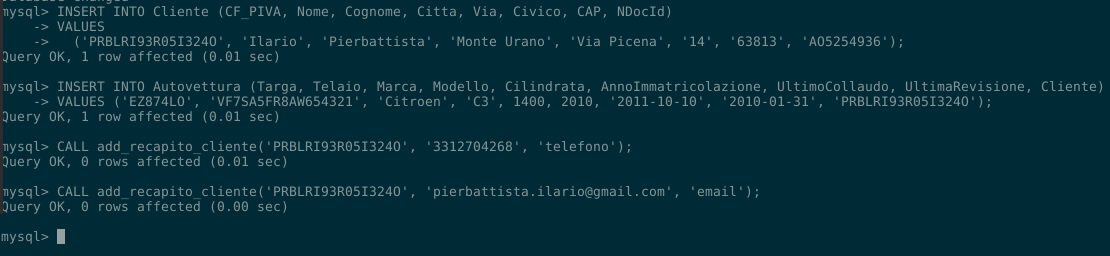
\includegraphics[width=15cm]{images/screenshots/nuovo_cliente.png}
        \end{figure}

        \begin{figure}[H]
          \centering
          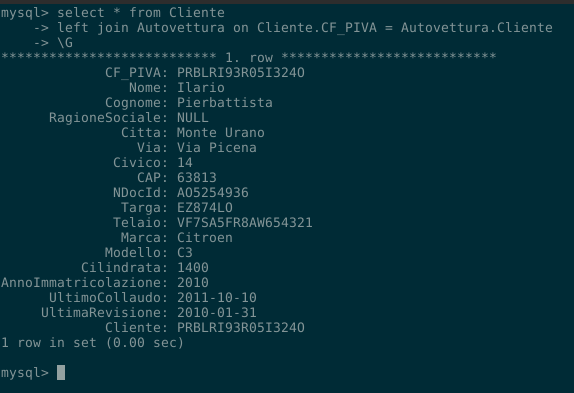
\includegraphics[width=9cm]{images/screenshots/show_cliente_autovettura.png}
        \end{figure}

			L'aggiunta di un recapito ad un cliente è un'operazione molto frequente. Per questo è stata creata una procedura che si occupa dell'inserimento e dell'associazione dello stesso:
				\begin{lstlisting}
CREATE PROCEDURE add_recapito_cliente(
  IN cf_piva  VARCHAR(16),
     recapito VARCHAR(200),
     tipo     ENUM('telefono',
                   'fax',
                   'tel_fax',
                   'sito_web',
                   'email')
)
  BEGIN
    DECLARE EXIT HANDLER FOR SQLEXCEPTION
    BEGIN
      ROLLBACK;
      /* La procedura throw_error si occupa di lanciare 
       * un segnale d'errore con codice 45000
       * e con il messaggio specificato come argomento
       */
      CALL throw_error('Recapito già registrato');
    END;
    START TRANSACTION;
    INSERT INTO Recapito (Recapito, Tipo) VALUES (recapito, tipo);
    SELECT LAST_INSERT_ID()
    INTO @last_id;
    INSERT INTO RubricaCliente (Recapito, Cliente) VALUES (@last_id, cf_piva);
    COMMIT;
  END;;
				\end{lstlisting}

        \begin{figure}[H]
          \centering
          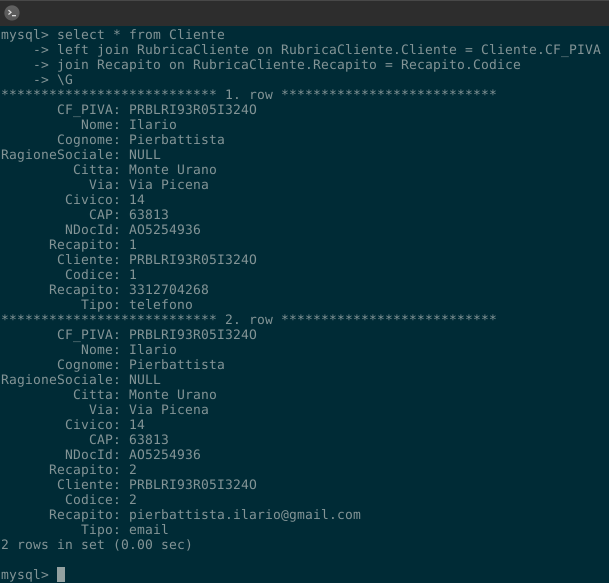
\includegraphics[width=9cm]{images/screenshots/show_cliente_rubrica.png}
        \end{figure}


			\subsubsection{Inserimento di un nuovo fornitore}
				All'inserimento di un nuovo fornitore corrisponde l'inserimento dei relativi recapiti.
				\begin{lstlisting}
/** Inserimento del fornitore */
INSERT INTO Fornitore (PIVA, RagioneSociale, TempiConsegna,
	ModPagamento, IBAN, Citta, Via, Civico, CAP) 
VALUES (...);

/** Associazione di un recapito inserito al fornitore
	(L'operazione di inserimento di un nuovo recapito
	è identica a quella presentata nel caso d'uso 
	precedente) */
INSERT INTO RubricaFornitore (Recapito, Fornitore)
VALUES (<Codice del recapito>, <PIVA del fornitore>);
				\end{lstlisting}

				Come nel caso precedente, anche per il fornitore esiste una procedura per l'aggiunta e l'associazione di un recapito.
				Gli inserimenti diventano molto più compatti:

				\begin{lstlisting}
CALL add_recapito_fornitore(<PIV del fornitore>,
	<recapito>, <tipo del recapito>);
				\end{lstlisting}

        Vista la semplicità di queste operazioni, non crediamo sia necessario allegare degli screenshot che ne testimonino la corretta esecuzione.


			\subsubsection{Inserimento di un nuovo operatore}
				Anche in questo caso bisognerà aggiungere uno o più recapiti a quest'ultimo. Presentiamo inoltre anche l'istruzione per inserire un nuovo turno di lavoro.
				\begin{lstlisting}
/** Inserimento di un operatore con stipendio fisso */
INSERT INTO Operatore (CF, Nome, Cognome, Citta, Via, 
	Civico, CAP, DataNasc, ComuneNasc, ProvinciaNasc, 
	Stipendio, ModRiscossione, IBAN)
VALUES (...);

/** Inserimento di un operatore con retribuzione
	oraria */
INSERT INTO Operatore (CF, Nome, Cognome, Citta, Via,
	Civico, CAP, DataNasc, ComuneNasc, ProvinciaNasc, 
	RetribuzioneH, ModRiscossione, IBAN)
VALUES (...);

/** Inserimento di un nuovo turno di lavoro */
INSERT INTO Turno (Operatore, Data, OraInizio, OraFine)
VALUES (<CF dell'operatore>, ...);

/** Aggiunta di un recapito */
CALL add_recapito_operatore(<CF dell'operatore>, <recapito>, 
	<tipo di recapito>)
				\end{lstlisting}

        Considerata la semplicità e l'analogia con i casi precedenti, non crediamo sia necessario allegare degli screenshot.


			\subsubsection{Inserimento di un nuovo componente}
				\begin{lstlisting}
INSERT INTO Componente (Nome, QuantitaMin, Validita, 
	PrezzoVendita) 
VALUES (...);
				\end{lstlisting}


			\subsubsection{Inserimento di un nuovo ordine}
				Questa operazione si articola in più parti: innanzi tutto bisogna creare una nuova istanza nella relazione \emph{Ordine}, quindi creare le istanze relative alle forniture dell'ordine.

				\begin{lstlisting}
/** Creazione del nuovo ordine */
INSERT INTO Ordine (DataEmissione, Fornitore, Imponibile) 
VALUES (...);

/** Creazione delle nuove forniture */
INSERT INTO Fornitura (Quantita, Componente, 
	Ordine, PrezzoUnitario)
VALUES (...), ..., (...);
				\end{lstlisting}

				In fase di creazione dell'ordine, inoltre, non è strettamente necessario inserirne l'imponibile. Lo si può calcolare in un secondo momento in base alle forniture associategli:

				\begin{lstlisting}
/** Aggiornamento dell'imponibile dell'ordine in base
 *  alle forniture associate allo stesso.
 *  Utilizzo della funzione calc_imponibile_ordine
 */
UPDATE Ordine
SET Imponibile = calc_imponibile_ordine(<Codice ordine>)
WHERE Ordine.Codice = <Codice ordine>;
				\end{lstlisting}

				Di seguito il corpo della funzione che automatizza il calcolo dell'attributo imponibile.

				\begin{lstlisting}
/** Implementazione di calc_imponibile_ordine
 *  Il primo parametro è il codice dell'ordine 
 */
CREATE FUNCTION calc_imponibile_ordine(ordine INTEGER)
  RETURNS DECIMAL(10, 2)
  BEGIN
    DECLARE result DECIMAL(10, 2);
    SELECT SUM(Fornitura.PrezzoUnitario * Fornitura.Quantita)
    FROM Ordine
      JOIN Fornitura ON Ordine.Codice = Fornitura.Ordine
    WHERE Ordine.Codice = ordine
    INTO result;
    RETURN result;
  END;;
				\end{lstlisting}

				Al pagamento dell'ordine, sarà necessario inserire una nuova transazione per registrare il pagamento al fornitore;

				\begin{lstlisting}
INSERT INTO Transazione (Quota, Data) VALUES (...);
UPDATE Ordine
SET Ordine.Versamento = <Codice della transazione>,
WHERE Ordine.Codice = <Codice dell'ordine>;
				\end{lstlisting}

				Ricordiamo che l'ammontare di tale transazione corrisponde all'imponibile dell'ordine cui vengono sommate le imposte ed altre somme eventuali. Per calcolare tale valore velocemente, si può utilizzare la funzione \emph{calc\_transazione\_ordine}:

				\begin{lstlisting}
/** Inserimento di una nuova transazione
 *  calcolando in modo automatico la quota 
 */
INSERT INTO Transazione (Quota, Data)
VALUES (calc_transazione_ordine(<Codice ordine>, 0), <Data>);

/**
 * Corpo della funzione calc_transazione_ordine
 * ordine: Codice dell'ordine di cui calcolare
 * 		il totale
 * plus: Somma aggiuntiva da aggiungere eventualmente
 * 		al risultato finale.
 */
CREATE FUNCTION calc_transazione_ordine(ordine INTEGER, plus REAL)
  RETURNS DECIMAL(10, 2)
  BEGIN
    DECLARE result DECIMAL(10, 2);
    SELECT Imponibile * (-(1 + IVA()))
    FROM Ordine
    WHERE Codice = ordine
    INTO result;
    RETURN result + plus;
  END;;
				\end{lstlisting}

				Infine, alla consegna dell'ordine da parte del fornitore, bisogna registrare la data di consegna ed inserire le nuove forniture nel magazzino.

				\begin{lstlisting}
/** Per ogni fornitura dell'ordine */
INSERT INTO Magazzino (Componente, Fornitura, Quantita)
VALUES (...);

/** Registrazione della data di consegna */
UPDATE Ordine
SET Ordine.DataConsegna = <Data di Consegna>
WHERE Ordine.Codice = <Codice dell'ordine>;
				\end{lstlisting}

				Infine anche per l'inserimento delle nuove forniture in magazzino abbiamo preparato una procedura che automatizza tale processo.

				\begin{lstlisting}
CALL registra_ordine_magazzino(<Codice dell'ordine>);

/** Corpo della funzione registra_ordine_magazzino
 * ordine: Codice dell'ordine di cui inserire le
 * 		forniture in magazzino 
 */
CREATE PROCEDURE registra_ordine_magazzino(IN ordine INTEGER)
  BEGIN
    DECLARE done BOOLEAN DEFAULT FALSE;
    DECLARE componente_id INT;
    DECLARE fornitura_id INT;
    DECLARE quantita INT;
    DECLARE cur CURSOR FOR
      SELECT
        Fornitura.Codice,
        Fornitura.Componente,
        Fornitura.Quantita
      FROM Fornitura
      WHERE Fornitura.Ordine = ordine;
    DECLARE CONTINUE HANDLER FOR NOT FOUND SET done = 1;
    DECLARE EXIT HANDLER FOR SQLEXCEPTION
    BEGIN
      ROLLBACK;
      CALL throw_error('Errore nell''inserimento dell''ordine in magazzino');
    END;
    START TRANSACTION;
    OPEN cur;
    REPEAT
      FETCH cur
      INTO fornitura_id, componente_id, quantita;
      IF NOT done
      THEN
        INSERT INTO Magazzino (Componente, Fornitura, Quantita)
        VALUES (componente_id, fornitura_id, quantita);
      END IF;
    UNTIL done END REPEAT;
    CLOSE cur;
    COMMIT;
  END;;
				\end{lstlisting}


			\subsubsection{Inserimento di un nuovo preventivo}

				\begin{lstlisting}
/** Inserimento di un nuovo preventivo */
INSERT INTO Preventivo (DataEmissione, DataInizio, Categoria,
	Sintomi, SisAlimentazione, TempoStimato, CostoComponenti, 
	Manodopera, ServAggiuntivi, Autovettura)
VALUES (...);

/** Inserimento dei componenti previsti */
INSERT INTO Previsione (Componente, Preventivo, 
	Ubicazione, Quantita)
VALUES (...), ..., (...);
				\end{lstlisting}

				Il costo dei componenti previsti dal preventivo può essere calcolato automaticamente alla fine dell'inserimento dei componenti previsti nella tabella \emph{Previsione}. Per far ciò abbiamo implementato una funzione chiamata \emph{calc\_costo\_componenti\_preventivo}.
				Inoltre, alla stipulazione di un preventivo, si può lasciare un acconto che viene regolarmente registrato.

				\begin{lstlisting}
/** Calcolo automatico del costo dei componenti */
UPDATE Preventivo 
SET CostoComponenti = calc_costo_componenti_preventivo(<Codice preventivo>)
WHERE Preventivo.Codice = <Codice preventivo>;

/** Inserimento di un acconto */
INSERT INTO Transazione (Quota, Data)
VALUES (...);
UPDATE Preventivo
SET Acconto       = <Codice della Transazione>,
WHERE Preventivo.Codice = <Codice del preventivo>;

/** Corpo della funzione calc_costo_componenti_preventivo
 *  preventivo: Codice del preventivo di cui calcolare il 
 * 			costo dei componenti
 */
CREATE FUNCTION calc_costo_componenti_preventivo(preventivo INTEGER)
  RETURNS DECIMAL(10, 2)
  BEGIN
    DECLARE result DECIMAL(10, 2);
    SELECT SUM(Previsione.PrezzoUnitario * Previsione.Quantita)
    FROM Preventivo
      LEFT JOIN Previsione ON Preventivo.Codice = Previsione.Preventivo
    WHERE Preventivo.Codice = preventivo
    INTO result;
    RETURN result;
  END;;
				\end{lstlisting}


      \subsubsection{Inserimento di una nuova prestazione}
        Questo caso d'uso è abbastanza macchinoso. Per la prestazione inserita bisogna specificare quali componenti sono stati utilizzati e di quali forniture, quali operatori l'hanno eseguita, quindi bisogna stilare una nuova fattura. Bisogna inoltre aggiornare il magazzino, decrementando le quantità dei componenti utilizzati.
        Stilata la fattura, al momento del pagamento della stessa, si può inserire una nuova transazione e marcare la fattura come pagata.

        \begin{lstlisting}
/** Inserimento di una nuova fattura */
INSERT INTO Prestazione (Preventivo, TempiEsecuzione, Procedimento,
                         DataFine, Manodopera, ServAggiuntivi)
VALUES (...);

/** Inserimento delle forniture utilizzate */
INSERT INTO Utilizzo (Prestazione, Fornitura, Quantita)
VALUES (<Codice della prestazione>, 
  <Codice della fornitura>, <Quantita usata>);

/** Procedura di aggiornamento delle quantità in magazzino */
CALL update_quantita_magazzino(<Codice prestazione>);

/** Associazione degli operatori che hanno eseguito la prestazione */
INSERT INTO Occupazione (Prestazione, Operatore)
VALUES (<Codice della prestazione>, <CF dell'operatore>);

/** Calcolo del prossimo numero progressivo della fattura */
SET @num_fattura = next_fattura_num(<Anno>);
INSERT INTO Fattura (Numero, Anno, Imponibile, Sconto, Incentivi,
                     DataEmissione, DataScadenza, TipoPag,
                     StatoPag, SisPag, Prestazione)
VALUES (@num_fattura, <Anno>, ...);

/** Inserimento della transazione a pagamento avvenuto */
INSERT INTO Transazione (Quota, Data)
VALUES (...);

/** Aggiornamento della fattura, marcata come pagata */
UPDATE Fattura
SET
  StatoPag    = TRUE,
  Transazione = <Codice della transazione>
WHERE Fattura.Numero = @num_fattura AND Fattura.Anno = <Anno>;
        \end{lstlisting}

        Forniamo, per completezza, le implementazioni della funzione \emph{next\_fattura\_num} e della procedura \emph{update\_quantita\_magazzino}.

        \begin{lstlisting}
/** Implementazione di next_fattura_num
 *  Restituisce il numero progressivo per la fattura successiva
 *  da inserire.
 *  anno: Anno in cui si intende emettere la fattura
 */
CREATE FUNCTION next_fattura_num(anno INTEGER)
  RETURNS INTEGER
  BEGIN
    DECLARE num INTEGER DEFAULT NULL;
    SELECT Fattura.Numero
    INTO num
    FROM Fattura
    WHERE Fattura.Anno = anno
    ORDER BY Fattura.Numero DESC
    LIMIT 1;
    IF num IS NULL
    THEN
      SET num = 1;
    ELSE
      SET num = num + 1;
    END IF;
    RETURN num;
  END;;

/** Implementazione di update_quantita_magazzino
 *  Aggiorna le quantità delle fatture attive in magazzino
 *  in seguito all'utilizzo di alcune di queste in una 
 *  prestazione.
 *  prestazione: codice della prestazione
 */
CREATE PROCEDURE update_quantita_magazzino(IN prestazione INTEGER)
  BEGIN
    DECLARE done BOOLEAN DEFAULT FALSE;
    DECLARE fornitura_id INT;
    DECLARE quantita INT;
    DECLARE quantita_presente INT;
    DECLARE error_message VARCHAR(128) 
      DEFAULT 'Errore nell''aggiornamento del magazzino';
    DECLARE cur CURSOR FOR
      SELECT
        Utilizzo.Fornitura,
        Utilizzo.Quantita
      FROM Utilizzo
      WHERE Utilizzo.Prestazione = prestazione;
    DECLARE CONTINUE HANDLER FOR NOT FOUND SET done = 1;
    DECLARE EXIT HANDLER FOR SQLEXCEPTION
    BEGIN
      ROLLBACK;
      CALL throw_error(error_message);
    END;
    START TRANSACTION;
    OPEN cur;
    REPEAT
      FETCH cur
      INTO fornitura_id, quantita;
      IF NOT done
      THEN
        SELECT Magazzino.Quantita
        INTO quantita_presente
        FROM Magazzino
        WHERE Magazzino.Fornitura = fornitura_id;
        IF quantita_presente - quantita >= 0
        THEN
          UPDATE Magazzino
          SET Magazzino.Quantita = Magazzino.Quantita - quantita
          WHERE Magazzino.Fornitura = fornitura_id;
        ELSE
          SET error_message = 'La quantità di componenti'
            ' disponibili non è sufficiente';
          CALL throw_error(error_message);
        END IF;
      END IF;
    UNTIL done END REPEAT;
    CLOSE cur;
    COMMIT;
  END;;
        \end{lstlisting}

        \subsubsection{Implementazione delle altre operazioni}
          Le altre operazioni possono essere presentate in maniera molto più lineare, non essendo, come le precedenti, fortemente legate tra loro.

          \begin{description}
            
            \item[\ref{op:edit_cliente}] Modifica dei dati di un cliente. Ovviamente 
              \begin{lstlisting}
/** Modifica di un cliente senza partita iva */
UPDATE Cliente
SET CF_PIVA      = <Nuovo codice fiscale>,
  Nome           = <Nuovo nome>,
  Cognome        = <Nuovo cognome>,
  Citta          = <Nuova città>,
  Via            = <Nuova via>,
  Civico         = <Nuovo civico>,
  CAP            = <Nuovo CAP>,
  NDocId         = <Nuovo numero del documento d'identità>
WHERE Cliente.CF_PIVA = <Codice fiscale del cliente da modificare>;

/** Modifica di un cliente con partita iva */
UPDATE Cliente
SET CF_PIVA      = <Nuova partita iva>,
  RagioneSociale = <Nuova ragione sociale>,
  Citta          = <Nuova città>,
  Via            = <Nuova via>,
  Civico         = <Nuovo civico>,
  CAP            = <Nuovo CAP>,
WHERE Cliente.CF_PIVA = <Partita iva del cliente da modificare>;
              \end{lstlisting}
            
            \item[\ref{op:edit_fornitore}] Modifica dei dati di un fornitore.
              \begin{lstlisting}
UPDATE Fornitore
SET PIVA         = <Nuova partita iva del fornitore>,
  RagioneSociale = <Nuova ragione sociale>,
  TempiConsegna  = <Nuovi tempi di consegna>,
  ModPagamento   = <Nuova modalità di pagamento>,
  IBAN           = <Nuovo iban>,
  Citta          = <Nuova città>,
  Via            = <Nuova via>,
  Civico         = <Nuovo civico>,
  CAP            = <Nuovo CAP>
WHERE Fornitore.PIVA = <Partita iva del fornitore da modificare>;
              \end{lstlisting}

            \item[\ref{op:edit_operatore}] Modifica dei dati di un operatore.
              \begin{lstlisting}
/** Modifica dei dati di un generico operatore */
UPDATE Operatore
SET CF           = <Nuovo codice fiscale>,
  Nome           = <Nuovo nome>,
  Cognome        = <Nuovo cognome>,
  Citta          = <Nuova città>,
  Via            = <Nuova via>,
  Civico         = <Nuovo civico>,
  CAP            = <Nuovo CAP>,
  DataNasc       = <Nuova data di nascita>,
  ComuneNasc     = <Nuovo comune di nascita>,
  ProvinciaNasc  = <Nuova provincia di nascita>,
  Stipendio      = <Nuovo stipendio>,
  RetribuzioneH  = <Nuova retribuzione oraria>,
  ModRiscossione = <Nuova modalità di riscossione>,
  IBAN           = <Nuovo IBAN>
WHERE Operatore.CF = <Codice fiscale dell'operatore da modificare>;
              \end{lstlisting}

            \item[\ref{op:edit_componente}] Modifica del prezzo di vendita di un componente.
              \begin{lstlisting}
UPDATE Componente
SET PrezzoVendita = <Nuovo prezzo di vendita>
WHERE Componente.Codice = <Codice del componente>;
              \end{lstlisting}

            \item[\ref{op:show_collaudo}] Consultazione della data di ultimo collaudo per un'autovettura.
              \begin{lstlisting}
SELECT UltimoCollaudo
FROM Autovettura
WHERE Targa = <Targa dell'auto>;
              \end{lstlisting}
              
              Inoltre, può essere utile avere una lista di tutte le auto registrate che in tempi brevi necessiteranno nuovamente del collaudo, in modo da poter facilmente repererne i proprietari.

              \begin{lstlisting}
/** Lista delle autovetture (con relativi proprietari)
 *  che necessitano di un nuovo collaudo entro 14 giorni.
 */
SELECT
  Autovettura.Targa,
  Autovettura.UltimoCollaudo,
  Cliente.Nome,
  Cliente.Cognome,
  Cliente.CF_PIVA
FROM Autovettura
  JOIN (
         SELECT
           Autovettura.Targa,
           DATEDIFF(
               CURRENT_DATE(),
               DATE_ADD(Autovettura.UltimoCollaudo, INTERVAL 5 YEAR)
           ) AS date_difference
         FROM Autovettura
       ) AS a ON a.Targa = Autovettura.Targa
  JOIN Cliente ON Cliente.CF_PIVA = Autovettura.Cliente
WHERE a.date_difference > - 14;
              \end{lstlisting}

              \begin{figure}[H]
                \centering
                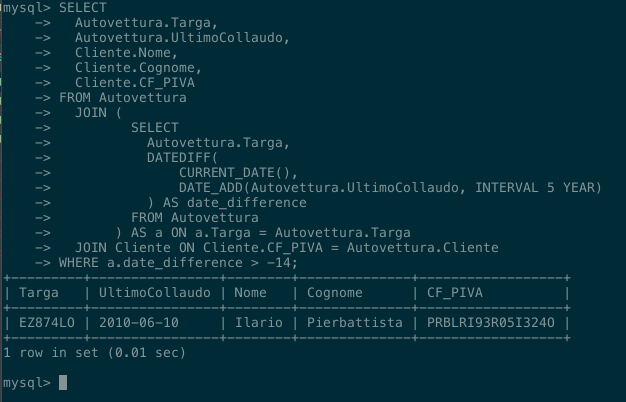
\includegraphics[width=9cm]{images/screenshots/list_collaudo_scadenza.png}
              \end{figure}


            \item[\ref{op:show_revisione}] Consultazione della data di ultima revisione per un'autovettura.
              \begin{lstlisting}
SELECT UltimaRevisione
FROM Autovettura
WHERE Targa = <Targa dell'autovettura>;
              \end{lstlisting}

              Analogamente al caso precedente è utile avere una lista delle autovetture la cui scadenza della revisione è prossima. Vista la forte analogia con il caso precedente, non riportiamo alcuno screenshot.
              \begin{lstlisting}
/** Lista delle autovetture (con relativi proprietari)
 *  che necessitano di una nuova revisione entro 14 giorni.
 */
SELECT
  Autovettura.Targa,
  Autovettura.UltimaRevisione,
  Cliente.Nome,
  Cliente.Cognome,
  Cliente.CF_PIVA
FROM Autovettura
  JOIN (
         SELECT
           Autovettura.Targa,
           DATEDIFF(
               CURRENT_DATE(),
               DATE_ADD(Autovettura.UltimaRevisione, INTERVAL 5 YEAR)
           ) AS date_difference
         FROM Autovettura
       ) AS a ON a.Targa = Autovettura.Targa
  JOIN Cliente ON Cliente.CF_PIVA = Autovettura.Cliente
WHERE a.date_difference > -14;
              \end{lstlisting}

            \item[\ref{op:show_fattura}] La visualizzazione dei dati di una fattura si articola in due fasi. La prima fase prevedere l'estrazione dei dati per stilare l'intestazione della fattura e la parte relativa agli importi.

            Ogni fattura nella sezione dedicata agli importi dovrà contenere l'\emph{imponibile Lordo}, lo \emph{sconto} in percentuale, l'\emph{Importo dello sconto}, l'\emph{imponibile netto}, l'ammontare delle \emph{imposte}, il valore di eventuali \emph{incentivi}, il \emph{totale}, il valore di un eventuale \emph{acconto} e il \emph{totale al netto dell'acconto}.

            Disponiamo solamente dell'\emph{imponibile netto} (attributo \emph{Imponibile} di \emph{Fattura}), del valore percentuale dello \emph{sconto} (attributo \emph{Sconto} di \emph{Fattura}), del valore degli \emph{incentivi} (attributo \emph{Incentivi} di \emph{Fattura}) e del valore dell'\emph{acconto} (attributo \emph{Quota} di \emph{Transazione}).

            Siano $i$, $s$, $A$, $D$, rispettivamente l'\emph{imponibile netto}, lo \emph{sconto percetuale}, l'\emph{acconto}, gli \emph{incentivi}. Sia inoltre $IVA$ l'ammontare in percentuale dell'iva.

            Sia $I$ l'\emph{imponibile lordo}, l'equazione \ref{eq:imponibile_lordo} fornisce la relazione con i parametri conosciuti.
            \begin{equation}
              \label{eq:imponibile_lordo}
              i = (1 - \frac{s}{100})\cdot I \Rightarrow I = \frac{i}{1 - \frac{s}{100}} \\
              \Rightarrow I = \frac{100 \cdot i}{100 - s} 
            \end{equation}

            Sia $S$ l'\emph{importo dello sconto}:
            \begin{equation}
              \label{eq:importo_sconto}
              I = i + S \Rightarrow S = i\cdot \left( \frac{100}{100 - s} - 1 \right) \\
              \Rightarrow S = i \cdot \left( \frac{s}{100 - s} \right)
            \end{equation}

            Sia $T$ il valore delle imposte:
            \begin{equation}
              \label{eq:imposte}
              T = i \cdot \frac{IVA}{100}
            \end{equation}

            Sia $TOT$ il \emph{totale lordo}:
            \begin{equation}
              \label{eq:totale_lordo}
              TOT = i + T - D
            \end{equation}

            Sia $tot$ il \emph{totale netto}:
            \begin{equation}
              \label{eq:totale_netto}
              tot = TOT - A
            \end{equation}

            Si assume che l'iva sia al $22\%$.

              \begin{lstlisting}
SELECT
  Fattura.Numero,
  Fattura.Anno,
  Fattura.DataEmissione,
  Fattura.SisPag,
  Cliente.Nome,
  Cliente.Cognome,
  Cliente.Citta,
  Cliente.Via,
  Cliente.Civico,
  Cliente.CAP,
  Autovettura.Targa,
  IFNULL(p.CostoComponenti, 0)
    AS CostoComponenti,
  Prestazione.Manodopera,
  Prestazione.ServAggiuntivi,
  f.ImponibileLordo,
  Fattura.Sconto,
  f.ImportoSconto,
  Fattura.Imponibile 
    AS ImponibileNetto,
  f.Imposte,
  Fattura.Incentivi,
  Fattura.Imponibile + f.Imposte - Fattura.Incentivi 
    AS Totale,
  IFNULL(Transazione.Quota, 0)
    AS RitenutaAcconto,
  Fattura.Imponibile + f.Imposte - Fattura.Incentivi - IFNULL(Transazione.Quota, 0) 
    AS TotaleNetto
FROM Fattura
  JOIN Prestazione ON Prestazione.Preventivo = Fattura.Prestazione
  JOIN Preventivo ON Preventivo.Codice = Prestazione.Preventivo
  LEFT JOIN Transazione ON Transazione.Codice = Preventivo.Acconto
  JOIN Autovettura ON Autovettura.Targa = Preventivo.Autovettura
  JOIN Cliente ON Cliente.CF_PIVA = Autovettura.Cliente
  LEFT JOIN (SELECT
               Utilizzo.Prestazione,
               SUM(Utilizzo.PrezzoUnitario * Utilizzo.Quantita) 
                AS CostoComponenti
             FROM Utilizzo
             GROUP BY Utilizzo.Prestazione
            ) 
          AS p 
        ON p.Prestazione = Prestazione.Preventivo
  JOIN (SELECT
          Fattura.Numero,
          Fattura.Anno,
          ROUND(Fattura.Imponibile * (100 / (100 - Fattura.Sconto)), 2)  
            AS ImponibileLordo,
          ROUND(Fattura.Imponibile * 0.22, 2)
            AS Imposte,
          ROUND(Fattura.Imponibile * (Fattura.Sconto / (100 - Fattura.Sconto)), 2) 
            AS ImportoSconto
        FROM Fattura) 
      AS f 
    ON Fattura.Numero = f.Numero AND Fattura.Anno = f.Anno
WHERE Fattura.Numero = <Numero della fattura> 
  AND Fattura.Anno = <Anno di emissione>;
              \end{lstlisting}

              \begin{figure}[H]
                \centering
                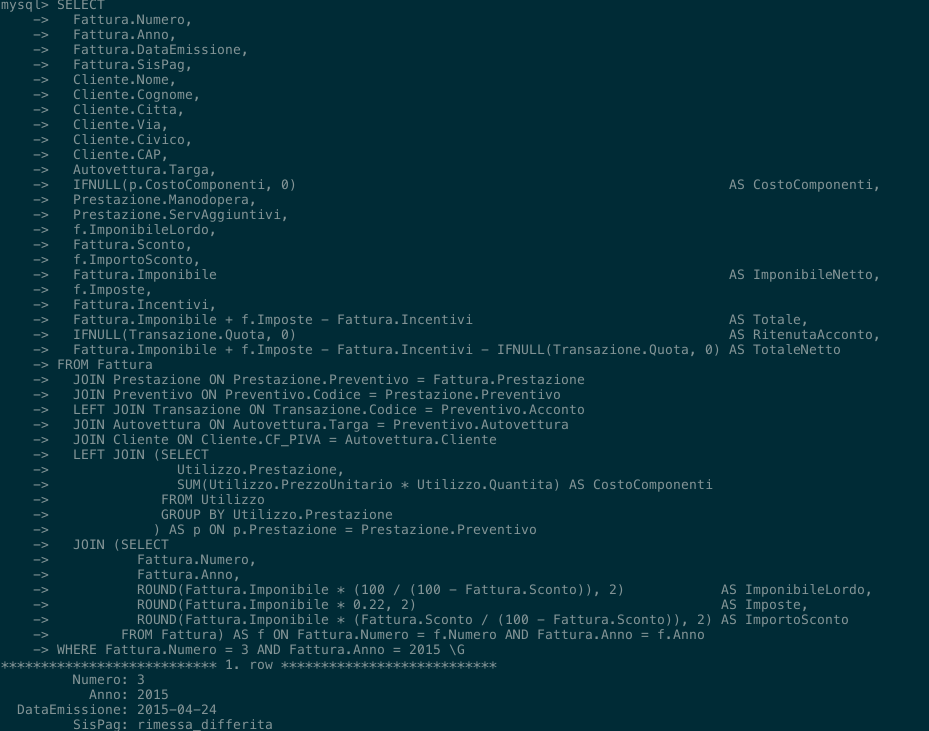
\includegraphics[width=14cm]{images/screenshots/show_intestazione_fattura_1.png}
              \end{figure}

              \begin{figure}[H]
                \centering
                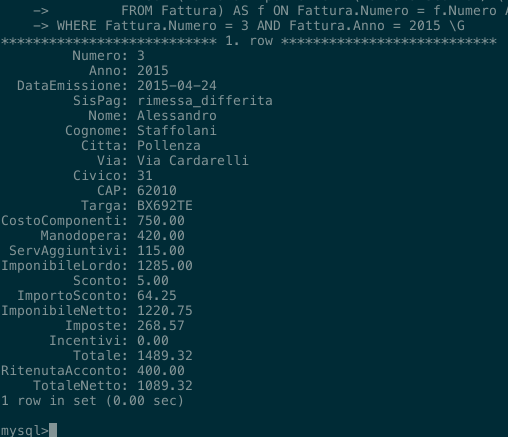
\includegraphics[width=10cm]{images/screenshots/show_intestazione_fattura_2.png}
              \end{figure}

              In alternativa, si può effettuare una selezione sulla vista \emph{FatturaView}, ottenendo lo stesso risultato con un'istruzione molto più compatta.

              \begin{lstlisting}
SELECT *
FROM FatturaView
WHERE Anno = <Anno di emissione> 
  AND Numero = <Numero della fattura>;
              \end{lstlisting}

              Alleghiamo uno screenshot che attesti l'equivalenza delle due istruzioni (quindi la corretta implementazione della vista, consultabile dal dump).

              \begin{figure}[H]
                \centering
                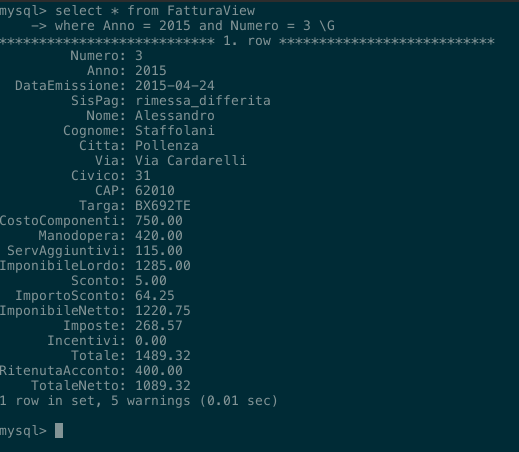
\includegraphics[width=10cm]{images/screenshots/show_fattura_view.png}
              \end{figure}

              La seconda fase della visualizzazione dei dati per stilare una fattura prevede la divisione dei costi dei singoli componenti utilizzati.

              \begin{lstlisting}
SELECT
  Componente.Codice as CodiceComponente,
  Componente.Nome,
  Utilizzo.Quantita,
  Utilizzo.PrezzoUnitario,
  Utilizzo.Quantita * Utilizzo.PrezzoUnitario AS PrezzoTotale
FROM Fattura
  JOIN Utilizzo ON Utilizzo.Prestazione = Fattura.Prestazione
  JOIN Fornitura ON Fornitura.Codice = Utilizzo.Fornitura
  JOIN Componente ON Componente.Codice = Fornitura.Componente
WHERE Anno = <Anno di emissione> 
  AND Numero = <Numero della fattura>;
              \end{lstlisting}

              \begin{figure}[H]
                \centering
                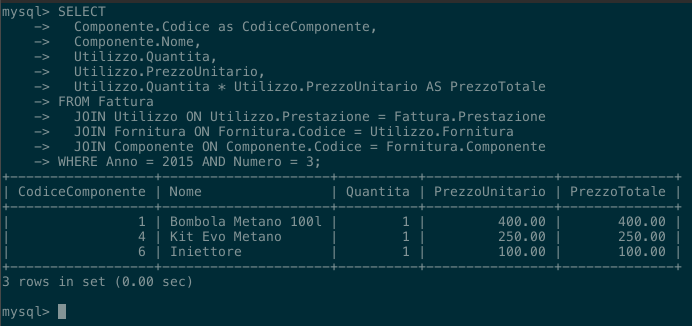
\includegraphics[width=10cm]{images/screenshots/show_componenti_fattura.png}
              \end{figure}

            \item[\ref{op:show_transazioni}] Consultazione delle transazioni avvenute in un certo periodo. La seguente istruzione, oltre a selezionare tutte le istanze interessate della tabella \emph{Transazione}, fornisce un'indicazione riguardante la natura della transazione e gli estremi per rintracciare l'istanza di \emph{Fattura}, \emph{Preventivo}, \emph{Ordine} o \emph{Operatore} ad essa associata.

              \begin{lstlisting}
SELECT
  Transazione.*,
  Preventivo.Codice                         AS Preventivo,
  CONCAT(Fattura.Numero, '/', Fattura.Anno) AS Fattura,
  Ordine.Codice                             AS Ordine,
  Stipendio.Operatore                       AS Operatore,
  CASE
  WHEN Preventivo.Acconto IS NOT NULL THEN 'acconto'
  WHEN Fattura.Transazione IS NOT NULL THEN 'pagamento prestazione'
  WHEN Ordine.Versamento IS NOT NULL THEN 'versamento fornitore'
  WHEN Stipendio.Transazione IS NOT NULL THEN 'stipendio'
  ELSE 'categoria non riconosciuta'
  END                                       AS Categoria
FROM Transazione
  LEFT JOIN Preventivo ON Transazione.Codice = Preventivo.Acconto
  LEFT JOIN Fattura ON Transazione.Codice = Fattura.Transazione
  LEFT JOIN Ordine ON Transazione.Codice = Ordine.Versamento
  LEFT JOIN Stipendio ON Transazione.Codice = Stipendio.Transazione
WHERE (Transazione.Data BETWEEN <Data di inizio>
  AND <Data di fine>)
ORDER BY Data DESC;
              \end{lstlisting}

              \begin{figure}[H]
                \centering
                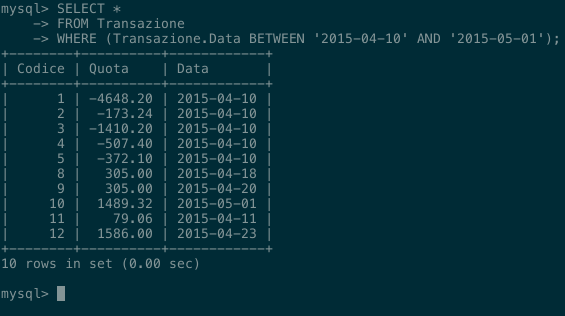
\includegraphics[width=12cm]{images/screenshots/show_transazioni.png}
              \end{figure}

            \item[\ref{op:show_riparazioni}] Consultazione della lista delle riparazioni

              \begin{lstlisting}
SELECT Prestazione.*
FROM Prestazione
JOIN Preventivo ON Preventivo.Codice = Prestazione.Preventivo
WHERE Categoria = 'riparazione';
              \end{lstlisting}

              \begin{figure}[H]
                \centering
                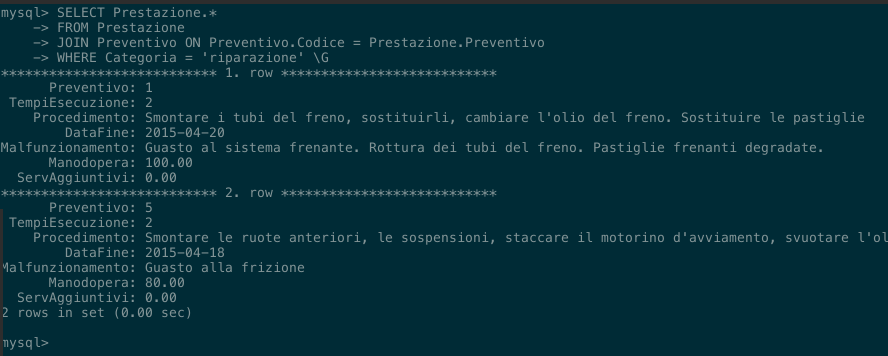
\includegraphics[width=12cm]{images/screenshots/list_riparazioni.png}
              \end{figure}

              Molto spesso può essere utile ricercare una riparazione in base al tipo di guasto riparato. Ad esempio, per ricercare i guasti riparati che coinvologono la frizione, si effettuerà una ricerca del tipo:

              \begin{lstlisting}
SELECT Prestazione.*
FROM Prestazione
  JOIN Preventivo ON Preventivo.Codice = Prestazione.Preventivo
WHERE Categoria = 'riparazione'
AND LOWER(Prestazione.Malfunzionamento) LIKE LOWER('%frizione%');
              \end{lstlisting}

              \begin{figure}[H]
                \centering
                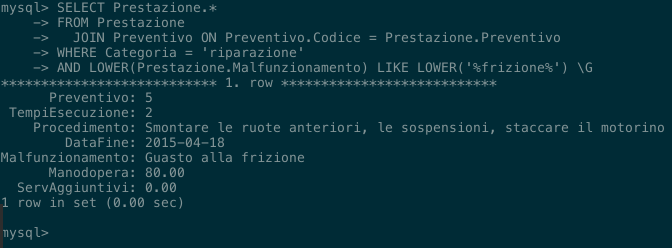
\includegraphics[width=12cm]{images/screenshots/search_riparazioni.png}
              \end{figure}

            \item[\ref{op:show_preventivi}] Consultazione della lista dei preventivi.

            È possibile visualizzare la lista di tutti i preventivi di una certa categoria:

              \begin{lstlisting}
SELECT *
FROM Preventivo
WHERE Categoria = 'installazione_impianto_gpl';
              \end{lstlisting}

              \begin{figure}[H]
                \centering
                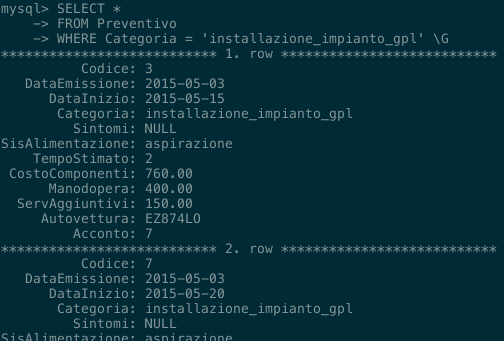
\includegraphics[width=8cm]{images/screenshots/search_preventivi_1.png}
              \end{figure}

            Di seguito presentiamo l'istruzione per ricercare il preventivo di una riparazione di un'autovettura con problemi ad inserire le marce:

              \begin{lstlisting}
SELECT *
FROM Preventivo
WHERE Categoria = 'riparazione' AND
      LOWER(Sintomi) LIKE LOWER('%marce%');
              \end{lstlisting}

              \begin{figure}[H]
                \centering
                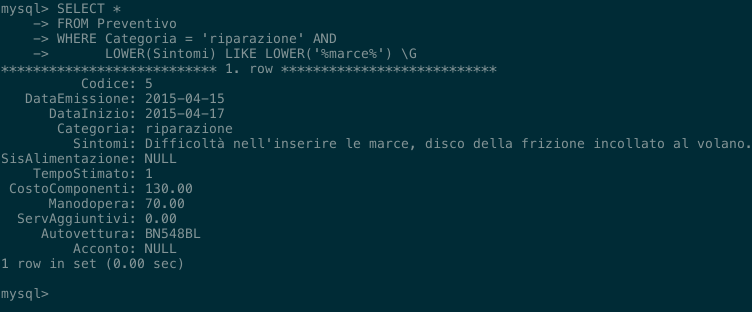
\includegraphics[width=10cm]{images/screenshots/search_preventivi_2.png}
              \end{figure}

            Possiamo effettuare ricerche ancora più restrittive, specificando anche la marca dell'auto ed il modello:

              \begin{lstlisting}
SELECT *
FROM Preventivo
  JOIN Autovettura ON Autovettura.Targa = Preventivo.Autovettura
WHERE Autovettura.Marca = 'Volkswagen'
      AND Autovettura.Modello = 'Golf'
      AND LOWER(Preventivo.Sintomi) LIKE '%freno%';
              \end{lstlisting}

              \begin{figure}[H]
                \centering
                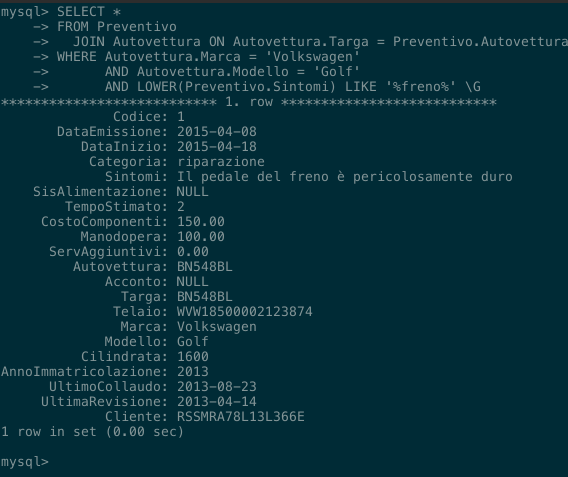
\includegraphics[width=9cm]{images/screenshots/search_preventivi_3.png}
              \end{figure}

            Le possibili combinazioni delle chiavi di ricerca sono tante e le query che ne verrebbero fuori sarebbero molto simili a quelle appena viste. Non ci soffermiamo oltre.

            \item[\ref{op:check_componente}] Controllo della disponibilità di un componente.

              \begin{lstlisting}
SELECT
  Componente.Codice,
  Componente.Nome,
  SUM(IFNULL(Magazzino.Quantita, 0)) AS QuantitaPresente
FROM Componente
  LEFT JOIN Magazzino ON Componente.Codice = Magazzino.Componente
WHERE Componente.Codice = <Codice del componente>
GROUP BY Componente.Codice;
              \end{lstlisting}

              \begin{figure}[H]
                \centering
                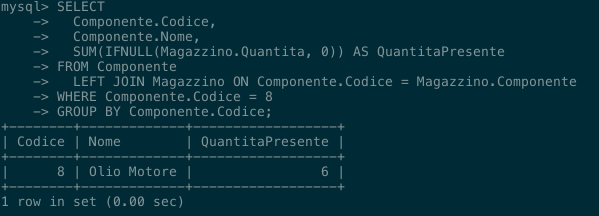
\includegraphics[width=10cm]{images/screenshots/check_componente.png}
              \end{figure}

            \item[\ref{op:check_turni}] Lista dei turni di un operatore durante un arco temporale.

              \begin{lstlisting}
SELECT *
FROM Turno
WHERE Turno.Operatore = <Codice fiscale dell'operatore>
      AND (Turno.Data BETWEEN <Data d'inizio>
      AND <Data di fine>)
ORDER BY Turno.Data ASC;
              \end{lstlisting}

              \begin{figure}[H]
                \centering
                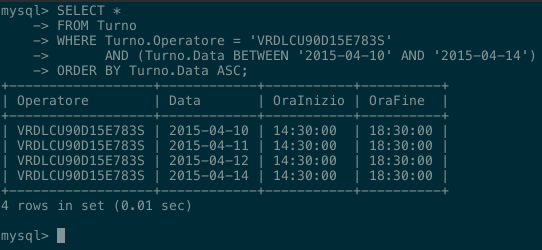
\includegraphics[width=8cm]{images/screenshots/show_turni.png}
              \end{figure}

            \item[\ref{op:list_componenti}] Lista dei componenti presenti in magazzino.

              \begin{lstlisting}
SELECT
  Componente.Codice,
  Componente.Nome,
  SUM(IFNULL(Magazzino.Quantita, 0)) AS QuantitaPresente
FROM Componente
  LEFT JOIN Magazzino ON Componente.Codice = Magazzino.Componente
GROUP BY Componente.Codice
HAVING QuantitaPresente > 0
ORDER BY Componente.Nome ASC;
              \end{lstlisting}

              \begin{figure}[H]
                \centering
                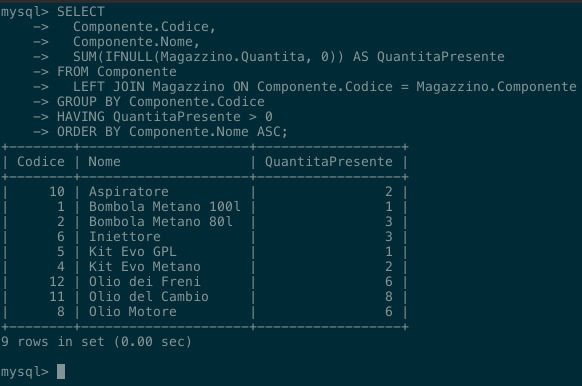
\includegraphics[width=10cm]{images/screenshots/list_componenti.png}
              \end{figure}

            \item[\ref{op:stats_componenti}] Lista dei componenti più usati. Viene calcolata la quantità totale dei componenti utilizzati in tutte le prestazioni registrate e la quantità media d'uso per ogni prestazione.

              \begin{lstlisting}
SELECT
  Componente.Codice,
  Componente.Nome,
  SUM(Utilizzo.Quantita)                      AS QuantitaUsata,
  COUNT(Prestazione)                          AS Prestazioni,
  SUM(Utilizzo.Quantita) / COUNT(Prestazione) AS QuantitaPrestazione
FROM Utilizzo
  JOIN Prestazione ON Prestazione.Preventivo = Utilizzo.Prestazione
  JOIN Fornitura ON Fornitura.Codice = Utilizzo.Fornitura
  JOIN Componente ON Componente.Codice = Fornitura.Componente
GROUP BY Componente
ORDER BY QuantitaUsata DESC
LIMIT <Quantità di componenti che si vuole visualizzare>;
              \end{lstlisting}

              \begin{figure}[H]
                \centering
                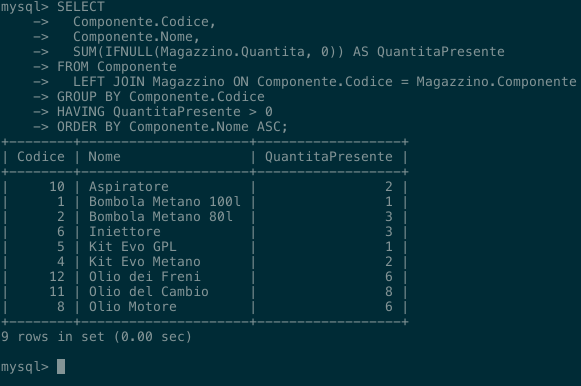
\includegraphics[width=12cm]{images/screenshots/stats_componenti.png}
              \end{figure}

            \item[\ref{op:tobuy_componenti}] Lista dei componenti che si dovrebbe acquistare nuovamente. Viene calcolata anche la quantità esatta da acquistare, oltre che la quantità attualmente presente.

              \begin{lstlisting}
SELECT
  Componente.Codice,
  Componente.Nome,
  Componente.QuantitaMin,
  m.QuantitaPresente,
  Componente.QuantitaMin - m.QuantitaPresente AS DaAcquistare
FROM Componente
  LEFT JOIN (SELECT
               Magazzino.Componente,
               SUM(IFNULL(Magazzino.Quantita, 0)) AS QuantitaPresente
             FROM Magazzino
             GROUP BY Magazzino.Componente
            ) AS m ON m.Componente = Componente.Codice
WHERE m.QuantitaPresente < Componente.QuantitaMin
ORDER BY Componente.Nome;
              \end{lstlisting}

              \begin{figure}[H]
                \centering
                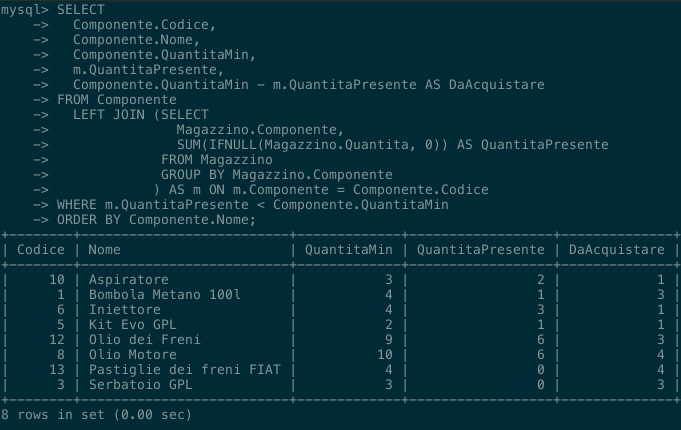
\includegraphics[width=12cm]{images/screenshots/tobuy_componenti.png}
              \end{figure}

            \item[\ref{op:show_recapiti_cliente}] Lista dei recapiti di un cliente.

              \begin{lstlisting}
SELECT
  Recapito.Recapito,
  Recapito.Tipo
FROM RubricaCliente
  JOIN Recapito ON Recapito.Codice = RubricaCliente.Recapito
WHERE RubricaCliente.Cliente = <CF_PIVA del cliente>;
              \end{lstlisting}

              \begin{figure}[H]
                \centering
                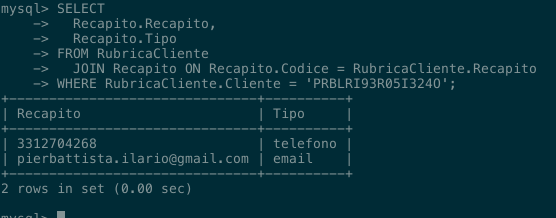
\includegraphics[width=10cm]{images/screenshots/list_recapiti_cliente.png}
              \end{figure}

              Per due operazioni successive, considerata la forte analogia, non saranno presentati screenshot.

            \item[\ref{op:show_recapiti_fornitore}] Lista dei recapiti di un fornitore.

              \begin{lstlisting}
SELECT
  Recapito.Recapito,
  Recapito.Tipo
FROM RubricaFornitore
  JOIN Recapito ON Recapito.Codice = RubricaFornitore.Recapito
WHERE RubricaFornitore.Fornitore = <PIVA del fornitore>;
              \end{lstlisting}

            \item[\ref{op:show_recapiti_operatore}] Lista dei recapiti di un operatore.

              \begin{lstlisting}
SELECT
  Recapito.Recapito,
  Recapito.Tipo
FROM RubricaOperatore
  JOIN Recapito ON Recapito.Codice = RubricaOperatore.Recapito
WHERE RubricaOperatore.Operatore = <CF dell'operatore>;
              \end{lstlisting}

            \item[\ref{op:list_fatture_pending}] Lista delle fatture che devono essere ancora pagate. Si calcolano anche i giorni rimanenti alla scadenza ed i giorni di ritardo nel pagamento al termine della scadenza.

              \begin{lstlisting}
SELECT
  Fattura.*,
  CASE
  WHEN DATEDIFF(DataScadenza, CURRENT_DATE()) < 0 THEN 0
  ELSE DATEDIFF(DataScadenza, CURRENT_DATE())
  END AS GiorniRimanenti,
  CASE
  WHEN DATEDIFF(CURRENT_DATE(), DataScadenza) < 0 THEN 0
  ELSE DATEDIFF(CURRENT_DATE(), DataScadenza)
  END AS GiorniRitardo
FROM Fattura
WHERE Fattura.StatoPag IS FALSE;
              \end{lstlisting}

              \begin{figure}[H]
                \centering
                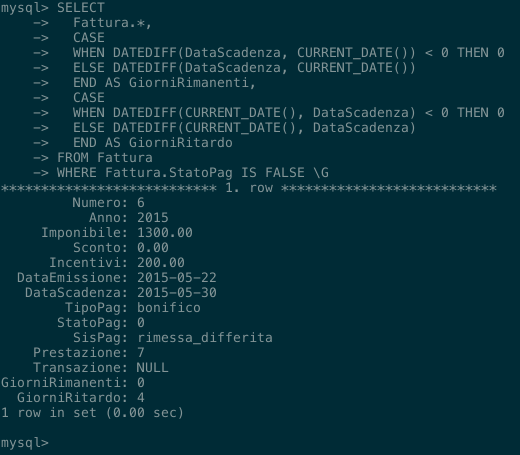
\includegraphics[width=10cm]{images/screenshots/list_fatture_pending.png}
              \end{figure}

            \item[\ref{op:list_ordini_pending}] Lista degli ordini che devono essere ancora consegnati.

              \begin{lstlisting}
SELECT
  Ordine.*,
  CASE
  WHEN DATEDIFF(
    CURRENT_DATE(), 
    DATE_ADD(DataEmissione, INTERVAL TempiConsegna DAY)
    ) < 0 THEN 0
  ELSE DATEDIFF(
    CURRENT_DATE(), 
    DATE_ADD(DataEmissione, INTERVAL TempiConsegna DAY)
    )
  END AS GiorniRitardo
FROM Ordine
  JOIN Fornitore ON Fornitore.PIVA = Ordine.Fornitore
WHERE DataConsegna IS NULL;
              \end{lstlisting}

              \begin{figure}[H]
                \centering
                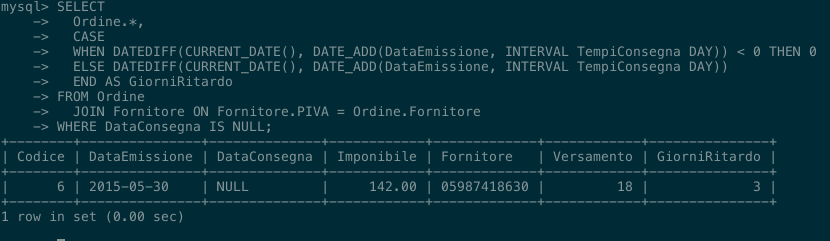
\includegraphics[width=14cm]{images/screenshots/list_ordini_pending.png}
              \end{figure}

            \item[\ref{op:todo_list}] Lista dei lavori da eseguire.

              \begin{lstlisting}
SELECT
  Preventivo.*,
  DATEDIFF(CURRENT_DATE(), Preventivo.DataInizio) AS GiorniRitardo
FROM Preventivo
  LEFT JOIN Fattura ON Fattura.Prestazione = Preventivo.Codice
WHERE DATEDIFF(CURRENT_DATE(), DataInizio) >= 0
      AND Fattura.Prestazione IS NULL;
              \end{lstlisting}

              \begin{figure}[H]
                \centering
                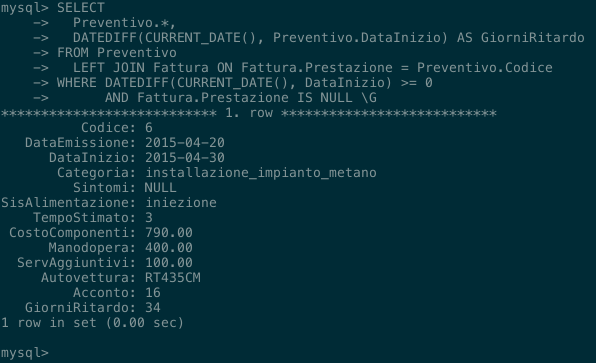
\includegraphics[width=12cm]{images/screenshots/todo_list.png}
              \end{figure}

            \item[\ref{op:calc_stipendio_operatore}] Calcolo dello stipendio degli operatori. Lo stipendio è mensile, tuttavia è necessario specificare manualmente gli estremi temporali di riferimento.
            È da notare che gli operatori con stipendio fisso (attributo \emph{Stipendio} di \emph{Operatore} diverso da null), riceveranno sempre lo stesso stipendio, mentre gli operatori che vengono retribuiti ad ore di lavoro (attributo \emph{RetribuzioneH} di \emph{Operatore}) riceveranno un compenso calcolato in base alla somma dei turni effettuati nell'arco temporale di riferimento.

              \begin{lstlisting}
SELECT
  Operatore.CF,
  Operatore.Nome,
  Operatore.Cognome,
  CASE
  WHEN Operatore.Stipendio IS NULL THEN Ore * RetribuzioneH
  ELSE Operatore.Stipendio
  END AS StipendioMensile
FROM Operatore
  JOIN (
         SELECT
           Turno.Operatore,
           SUM(ROUND(TIME_TO_SEC(TIMEDIFF(OraFine, OraInizio)) / 3600, 1)) AS Ore
         FROM Turno
         WHERE (Turno.Data BETWEEN '2015-04-01' AND '2015-05-01')
         GROUP BY Operatore
       ) AS t ON t.Operatore = Operatore.CF;
              \end{lstlisting}

              \begin{figure}[H]
                \centering
                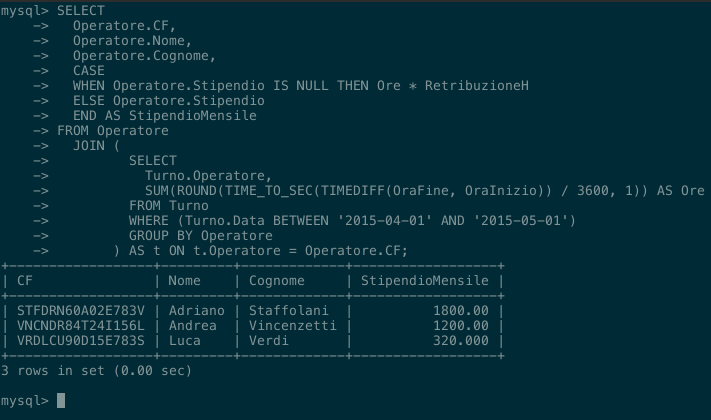
\includegraphics[width=12cm]{images/screenshots/calc_stipendio_operatore.png}
              \end{figure}

            \item[\ref{op:stats_prevetivi_prestazioni}] Scostamento tra i costi preventivati e quelli effettivi. Il costo delle prestazioni è stato messo a confronto con i costi preventivati, sia nella sua totalità, sia scorporandolo nelle voci di cui è composto. Inoltre è stato calcolato l'errore nella previsione di ogni voce, definito come la differenza tra l'effettivo e il preventivato (il segno stabilisce solamente la direzione dell'errore).

              \begin{lstlisting}
SELECT
  Preventivo.Codice,
  Preventivo.CostoComponenti                       AS ComponentiPrevisti,
  SUM(Utilizzo.PrezzoUnitario * Utilizzo.Quantita) AS ComponentiEffettivi,
  SUM(Utilizzo.PrezzoUnitario * Utilizzo.Quantita) -
  Preventivo.CostoComponenti
                                                   AS ErroreComponenti,
  Preventivo.Manodopera                            AS ManodoperaPrevista,
  Prestazione.Manodopera                           AS ManodoperaEffettiva,
  Prestazione.Manodopera - Preventivo.Manodopera   AS ErroreManodopera,
  Preventivo.ServAggiuntivi                        AS CostiAggiuntiviPrevisti,
  Prestazione.ServAggiuntivi                       AS CostiAggiuntiviEffettivi,
  Prestazione.ServAggiuntivi - Preventivo.ServAggiuntivi
                                                   AS ErroreCostiAggiunti,
  Preventivo.CostoComponenti + Preventivo.Manodopera +
  Preventivo.ServAggiuntivi
                                                   AS TotalePrevisto,
  SUM(Utilizzo.PrezzoUnitario * Utilizzo.Quantita) +
  Prestazione.Manodopera + Prestazione.ServAggiuntivi
                                                   AS TotaleEffettivo,
  SUM(Utilizzo.PrezzoUnitario * Utilizzo.Quantita) +
  Prestazione.Manodopera + Prestazione.ServAggiuntivi -
  (Preventivo.CostoComponenti + Preventivo.Manodopera +
   Preventivo.ServAggiuntivi)
                                                   AS ErroreTotale
FROM Preventivo
  JOIN Prestazione ON Preventivo.Codice = Prestazione.Preventivo
  JOIN Utilizzo ON Prestazione.Preventivo = Utilizzo.Prestazione
GROUP BY Prestazione;
              \end{lstlisting}

              \begin{figure}[H]
                \centering
                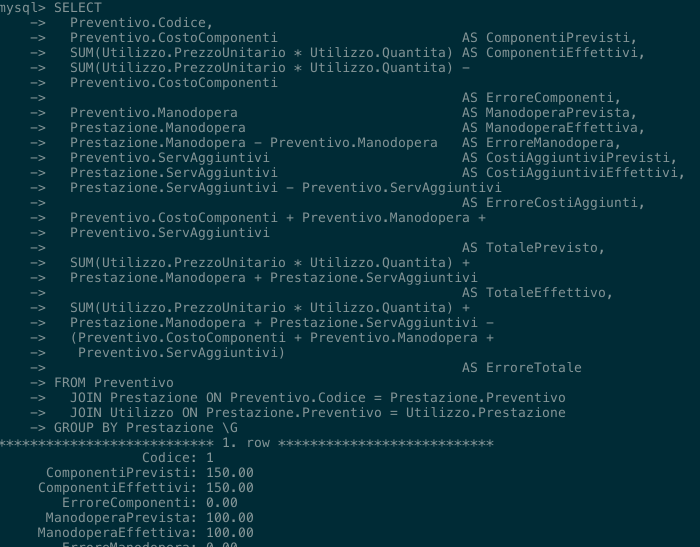
\includegraphics[width=12cm]{images/screenshots/scostamento_1.png}
              \end{figure}

              \begin{figure}[H]
                \centering
                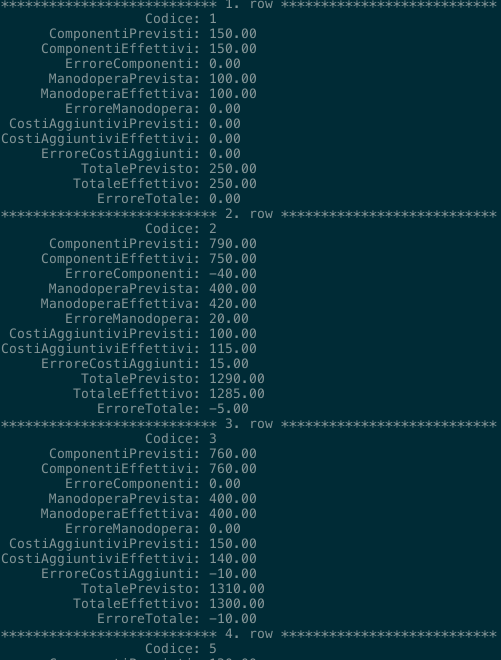
\includegraphics[width=8cm]{images/screenshots/scostamento_2.png}
              \end{figure}

            \item[\ref{op:stats_costi}] Variazione dei costi di un componente.

              \begin{lstlisting}
SELECT
  Fornitura.Componente,
  Fornitura.PrezzoUnitario AS PrezzoAcquisto,
  Ordine.DataEmissione
FROM Fornitura
  JOIN Ordine ON Ordine.Codice = Fornitura.Ordine
WHERE Componente = 2
ORDER BY DataEmissione DESC;
              \end{lstlisting}

              \begin{figure}[H]
                \centering
                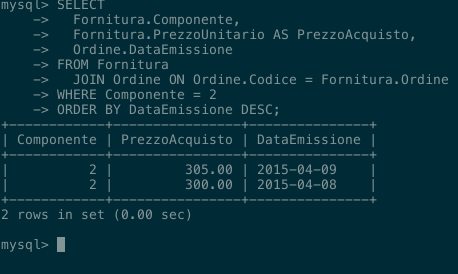
\includegraphics[width=8cm]{images/screenshots/stats_costi.png}
              \end{figure}

          \end{description}
